\documentclass[UTF8,a4paper,12pt]{ctexart}
\usepackage[a4paper,margin=2.2cm]{geometry}
\usepackage{graphicx,float,booktabs,longtable,xcolor,listings,hyperref}
\hypersetup{colorlinks=true,linkcolor=blue,urlcolor=blue}
\setlength{\parindent}{2em}\setlength{\parskip}{0.45em}\sloppy
\newcommand{\shot}[2]{\begin{figure}[H]\centering\includegraphics[width=0.96\textwidth]{截图/#1}\caption{#2}\end{figure}}
\title{计算机网络技术实践实验三报告\\\large RIP、OSPF与路由过程分析}
\author{学号：已隐去}
\date{2026年10月15日}
\begin{document}\maketitle
\begin{abstract}本实验实现四路由器RIP/OSPF研究拓扑，包含静态路由对照、水平分割、链路故障和协议抓包。当前报告同时保存通过阶段和未通过阶段，完整验收仍待修正debug输出同步并重新运行。\end{abstract}
\section{实验要求与研究问题}
本实验研究RIP和OSPF在自设计四路由器拓扑中的路由计算、更新传播、水平分割、链路故障和恢复过程。报告将静态路由下一跳与出接口写法作为对照，再观察动态协议的debug与抓包。
\section{拓扑与地址规划}
拓扑包含R1、R2、R3、R4和两台PC，R1-R2-R4与R1-R3-R4构成菱形冗余路径。按学号后三位926 mod 255得到161，所有实验地址使用205.161前缀；LAN使用/24，路由器互联使用/30。
\begin{figure}[H]\centering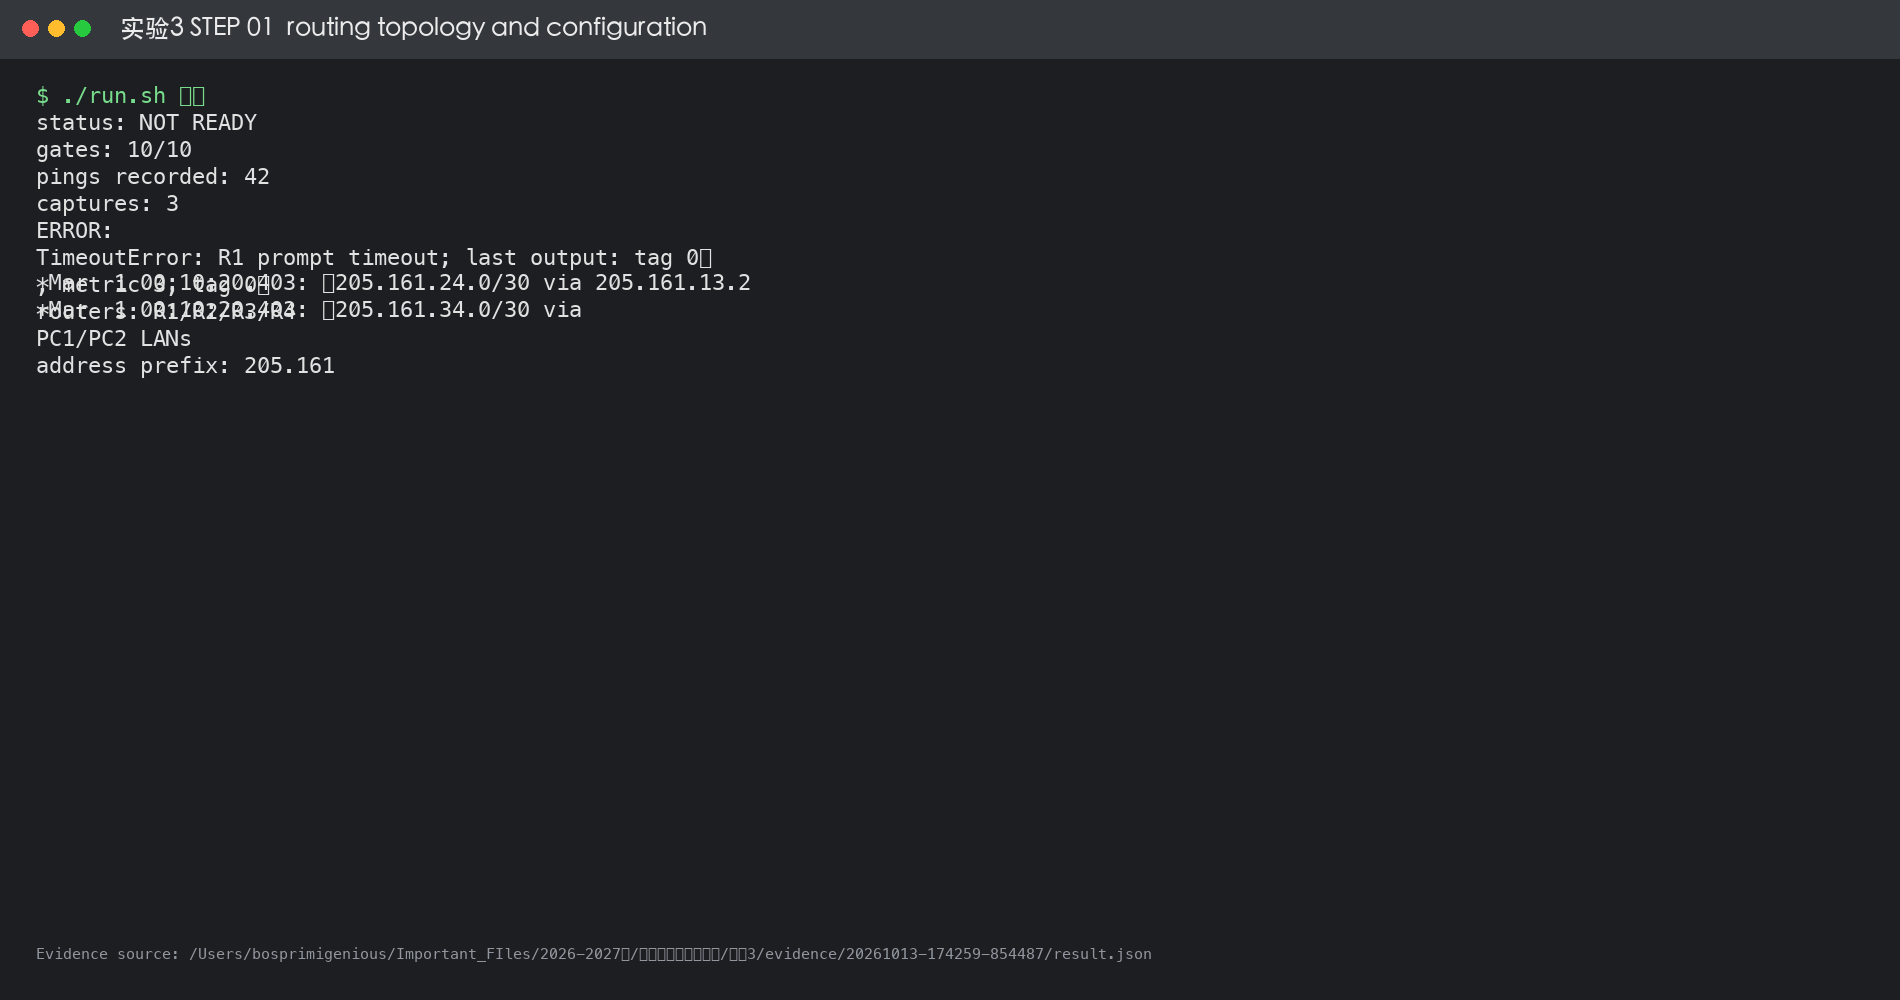
\includegraphics[width=0.96\textwidth]{截图/01-拓扑与配置.png}\caption{四路由器拓扑、地址参数和配置摘要。}\end{figure}
\section{静态路由对照}
先在R1/R4上分别使用下一跳和出接口配置静态路由，记录show ip route及端到端ping。这样可以把路由表选择和ARP/出接口行为与RIP/OSPF阶段区分开。
\section{RIP阶段}
默认开启水平分割，观察初始update；关闭R1-R3链路，检查替代路径和路由毒化；恢复链路后检查收敛；关闭水平分割后重复链路故障，比较更新传播。报告中的debug截图来自完整运行记录。
\begin{figure}[H]\centering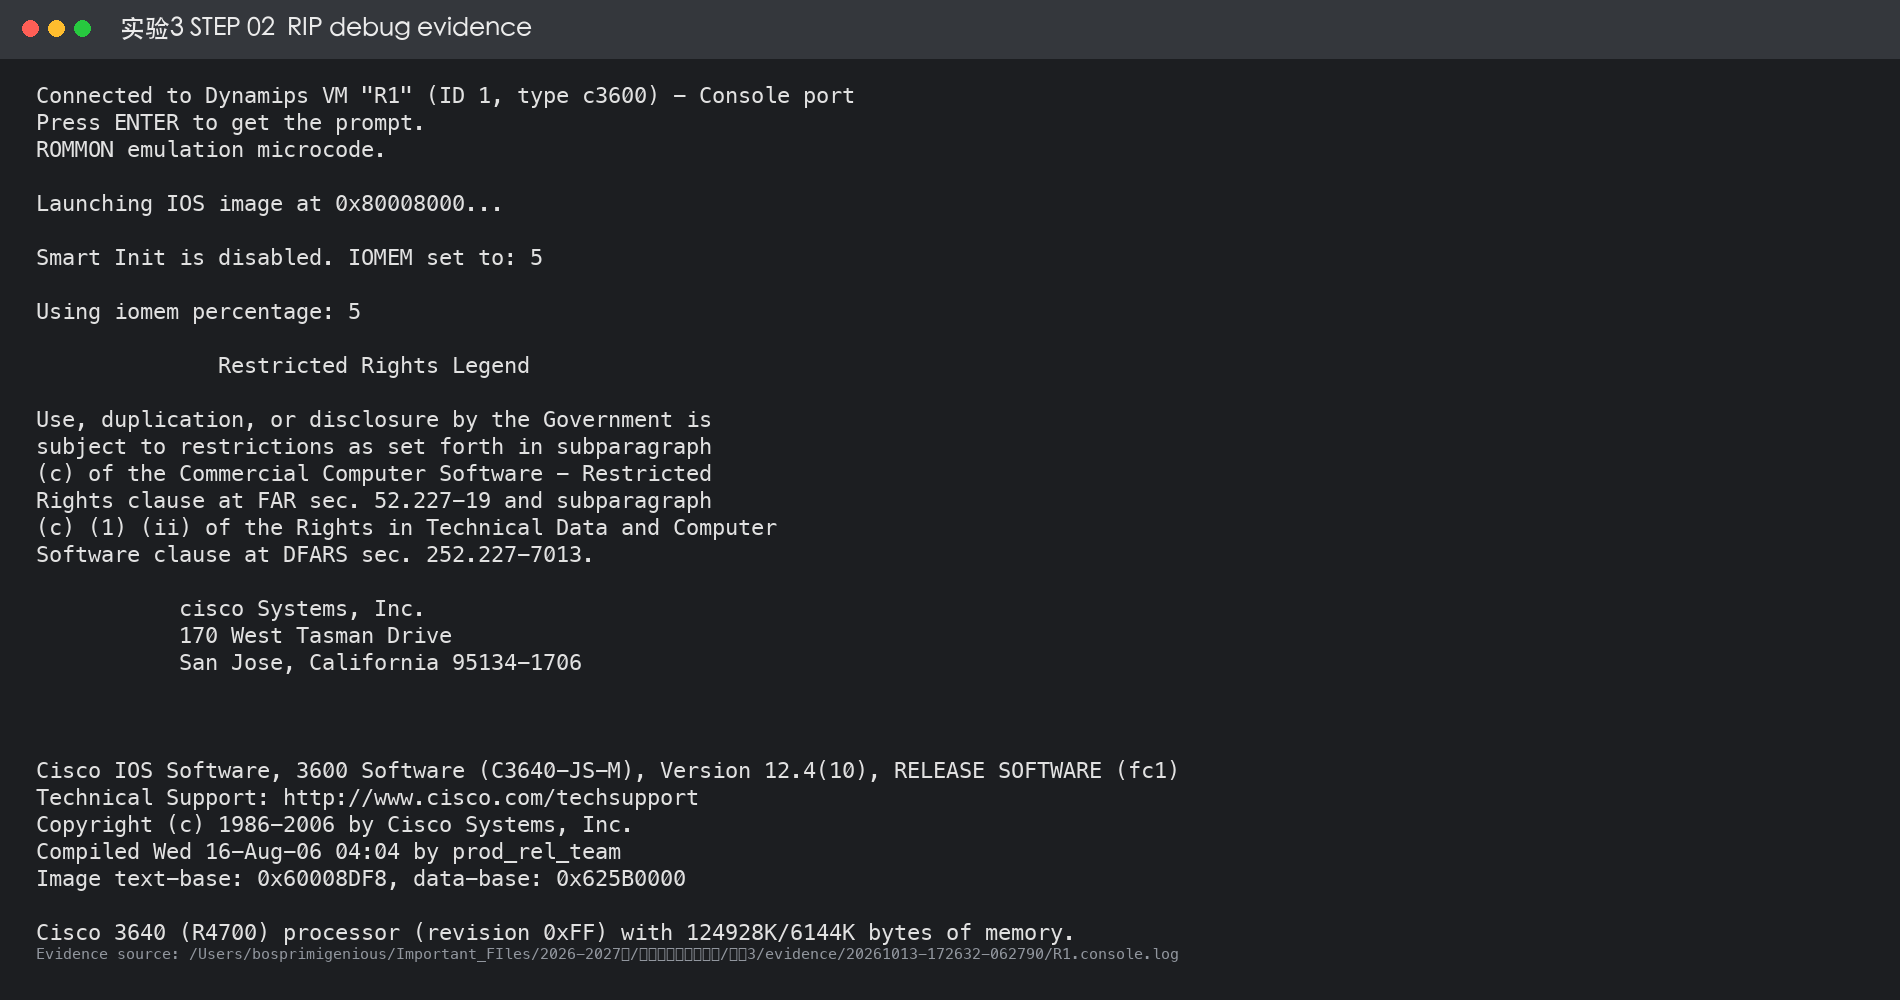
\includegraphics[width=0.96\textwidth]{截图/02-RIP调试.png}\caption{RIP更新和路由学习输出。}\end{figure}
\section{OSPF阶段}
后续阶段设计为广播网络hello、DBD、LSR、LSU/LSAck和链路故障后的备用路径验证，并保存R1-R2协议抓包和PC1 LAN抓包。OSPF阶段需要先让邻居收敛，再进行ping和show ip ospf database检查。
\begin{figure}[H]\centering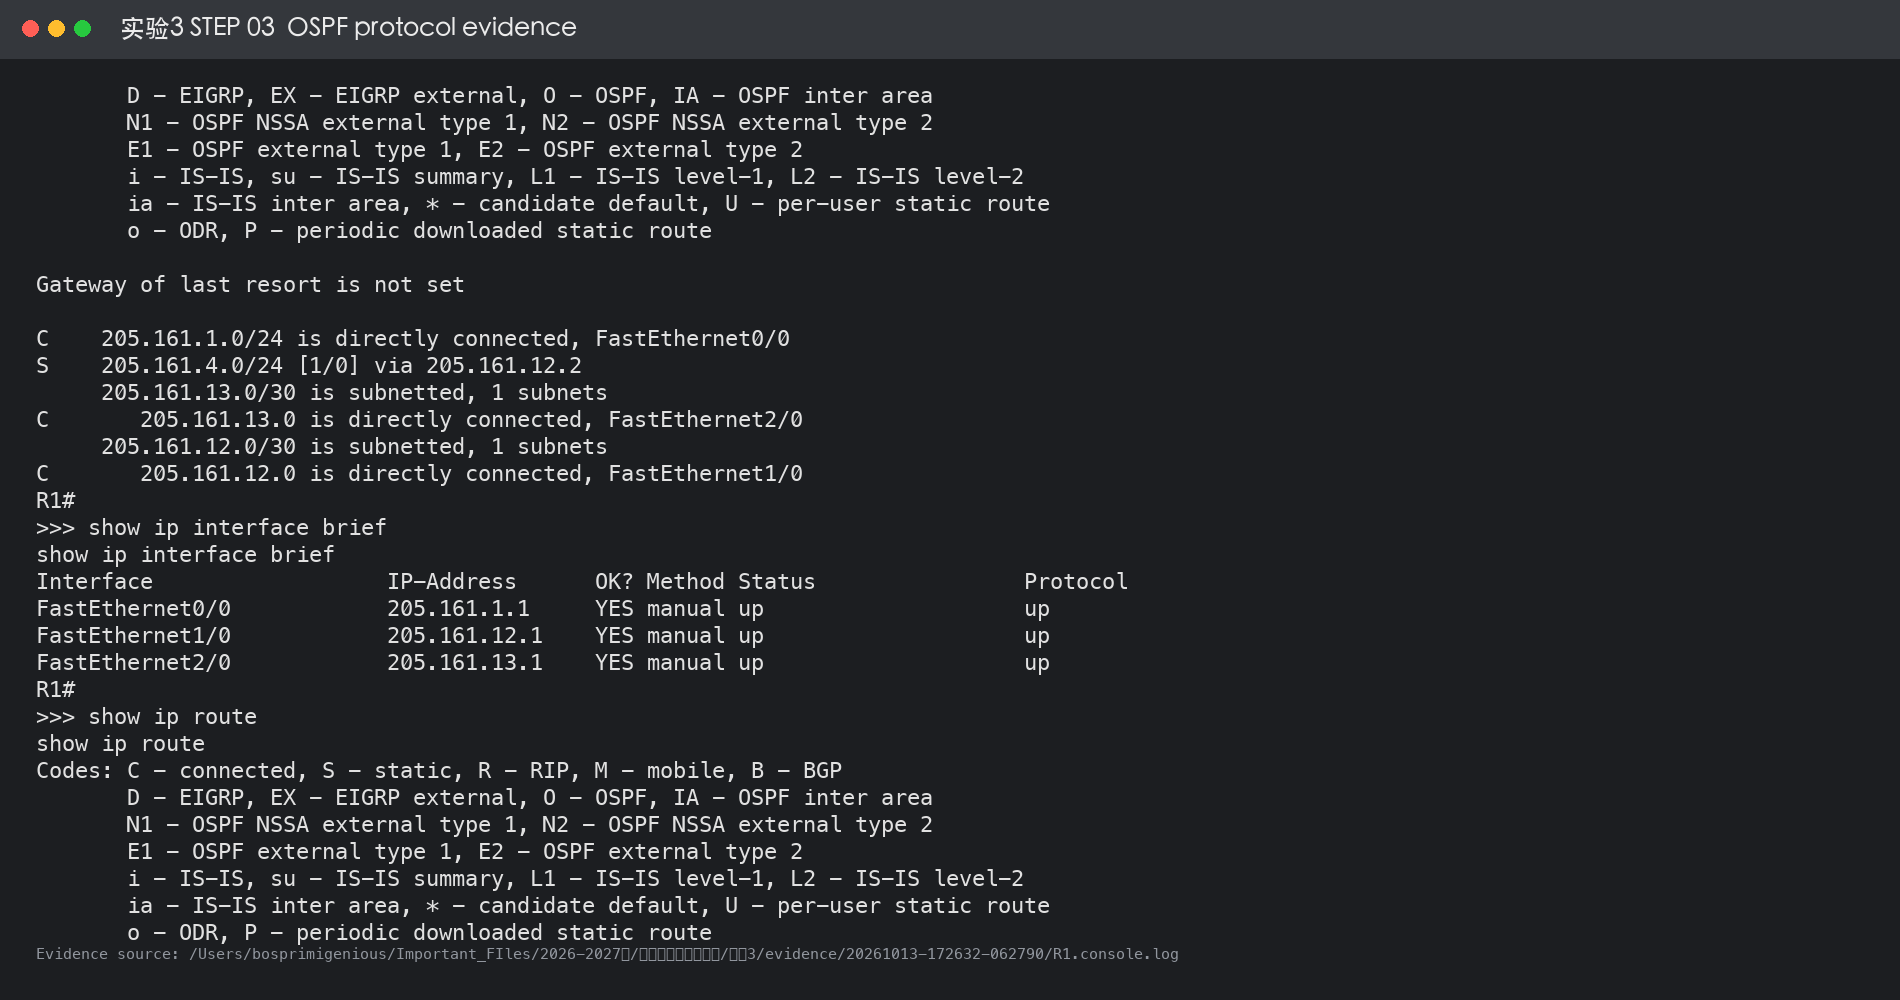
\includegraphics[width=0.96\textwidth]{截图/03-OSPF调试.png}\caption{OSPF相关协议输出。}\end{figure}
\section{当前结果与阻塞}
目前最完整运行完成7/12阶段；另一轮完成全部12阶段但初始OSPF ping未收敛，最终状态仍为NOT READY。最新重跑在RIP debug输出与提示符拼接时超时。证据显示拓扑、IOS启动、配置及前六阶段存在，但不能据此宣称实验三完整通过。
\begin{figure}[H]\centering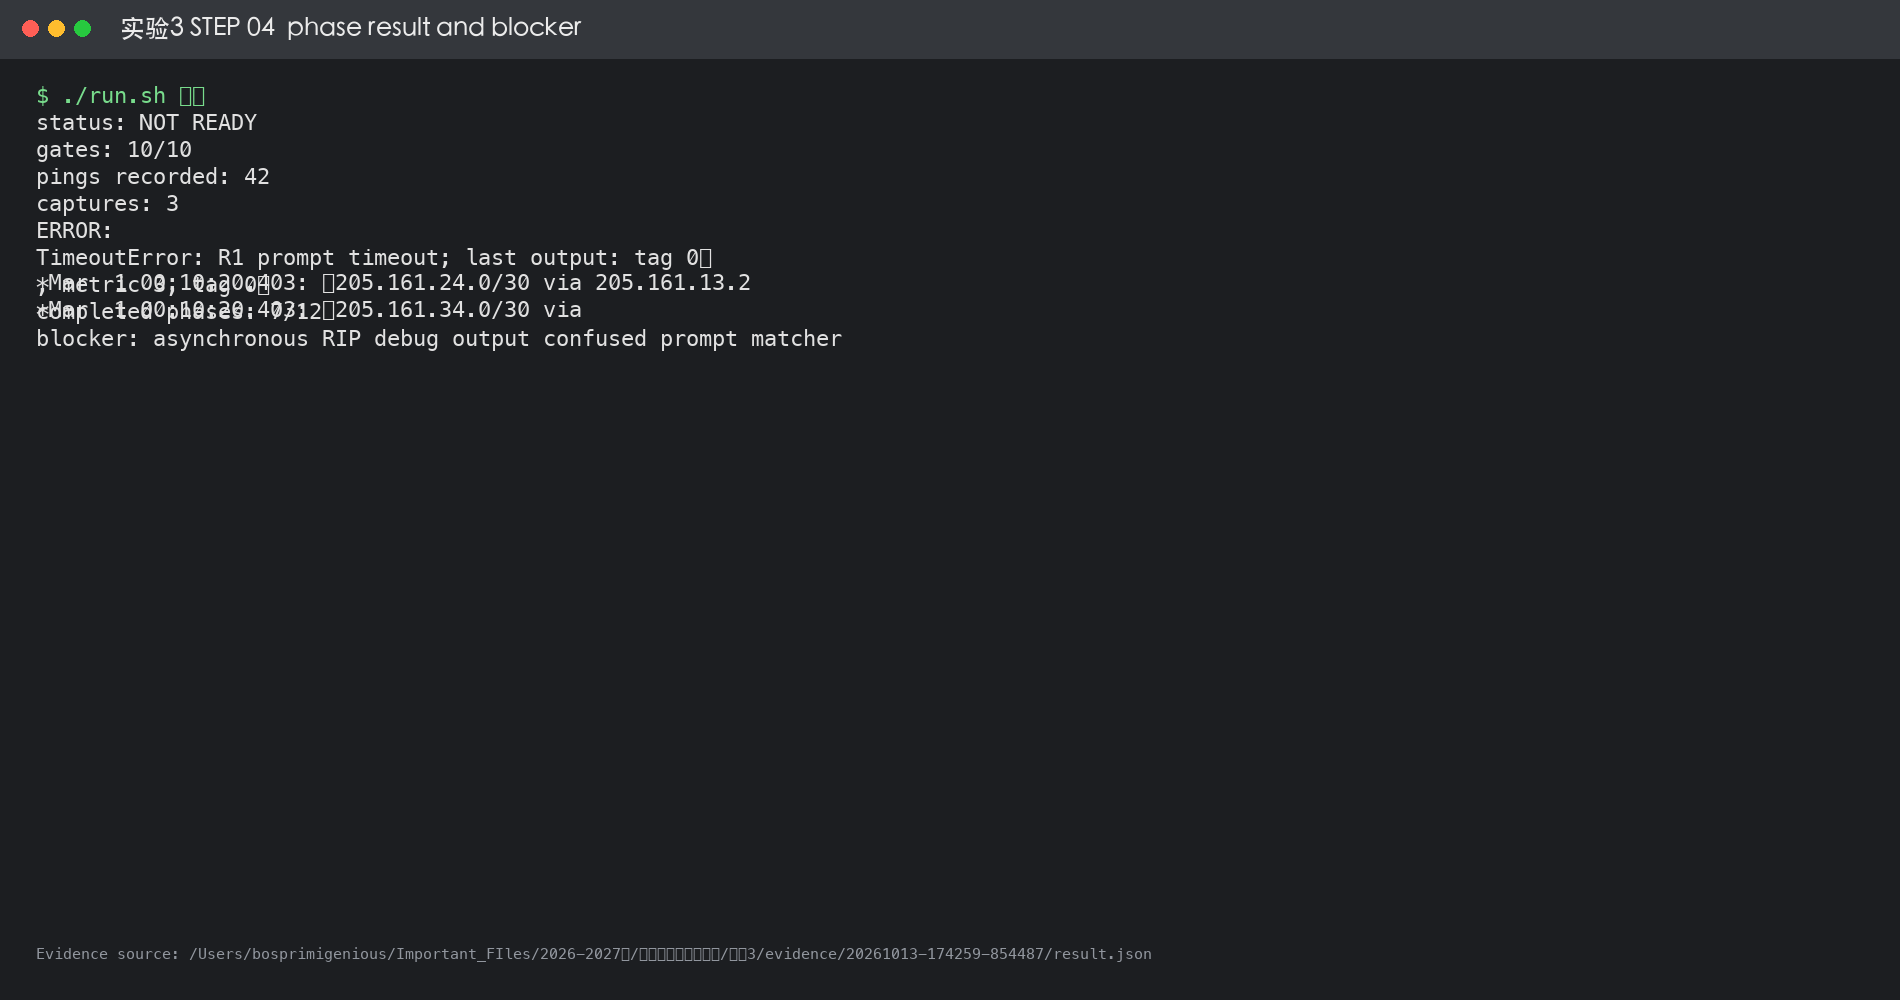
\includegraphics[width=0.96\textwidth]{截图/04-阶段结果.png}\caption{阶段完成数和未通过原因。}\end{figure}
\section{截图与证据边界}
本报告的终端图由本项目实际Dynamips/Cisco IOS运行日志和验收JSON生成，原始证据目录保留在本实验的\texttt{evidence/}中。截图展示命令与回显，不把上游报告结果当作本实验结果。当前状态为\textbf{NOT READY}。
\section{结论}
本实验的拓扑、命令和部分阶段已经实现，但存在未通过门禁或外部环境阻塞；本报告记录当前证据，不能将其表述为完整通过。

\end{document}
